\block{}{
 	{ \fontsize{40}{40}\selectfont 

	\section{Pré-traitement}
	À cette étape, j'ai utilisé la méthode Hough Transform de scikit-image pour détecter l'iris dans les images. Ensuite, j'ai appliqué la technique Warp Polar de scikit-image pour transformer l'iris circulaire détecté en rectangle.\cite{ref_4} J'ai, par la suite, retiré la partie noire (la pupille) de l’image rectangulaire.
	
	
	\section{Extraction des caractéristiques}
	Pour l'extraction des caractéristiques, j'ai utilisé la méthode GLCM. Elle permet d'analyser les textures en calculant les répartitions des différents des niveaux de gris dans l'image en se basant sur les positions relatives des pixels. À partir de cette matrice, certaines caractéristiques de texture comme le contraste, l'énergie, l'homogénéité, etc. peuvent être identifiées.\cite{ref_5}
	
	\section{Réduction de la dimensionnalité}
	La réduction de la dimensionnalité est un processus qui consiste à réduire considérablement le nombre de caractéristiques pour faciliter le processus d’entraînement.\cite{ref_1} La méthode que j'ai utilisée est la PCA de scikit-learn.
	
	\section{Processus de classification}
    Pour la classification, j'ai utilisée la méthode k-NN. La méthode des k voisins les plus proches (k-NN) consiste à trouver les k échantillons dont l’entrée est la plus proche d’une nouvelle entrée.
    
    \vspace{1em}
    \begin{center}
        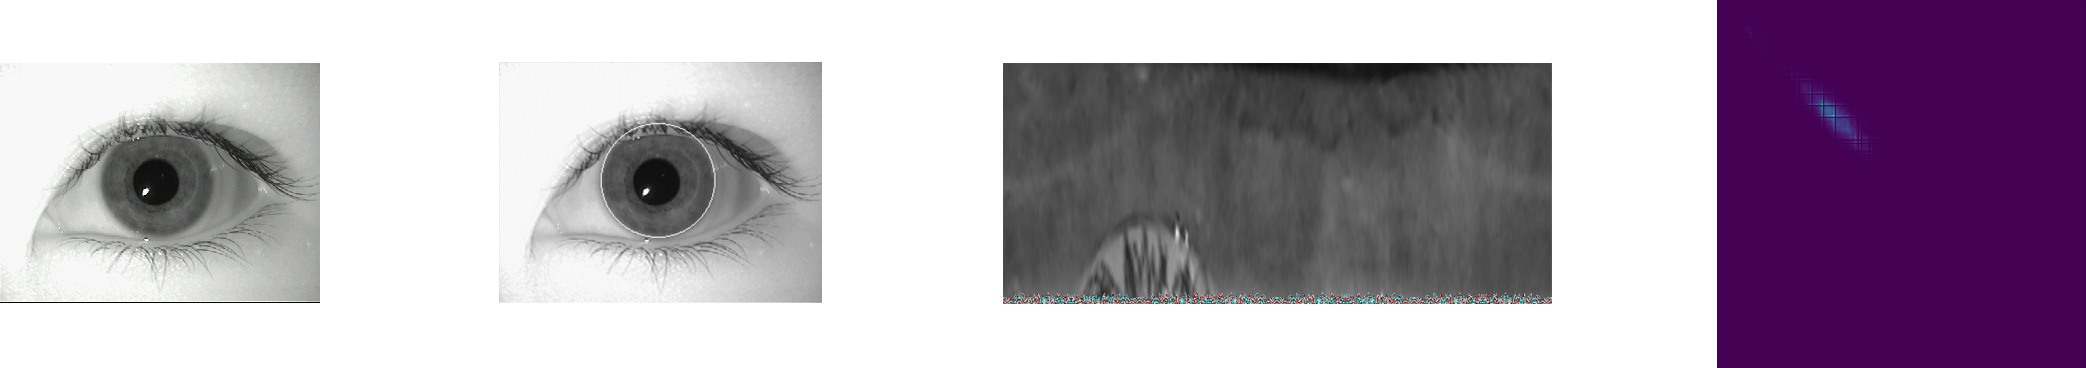
\includegraphics[width=0.9\linewidth]{processus}
        \captionof{figure}{Processus.}
    \end{center}
    \vspace{1em}
    
	}
}